% This file was created with tikzplotlib v0.10.1.
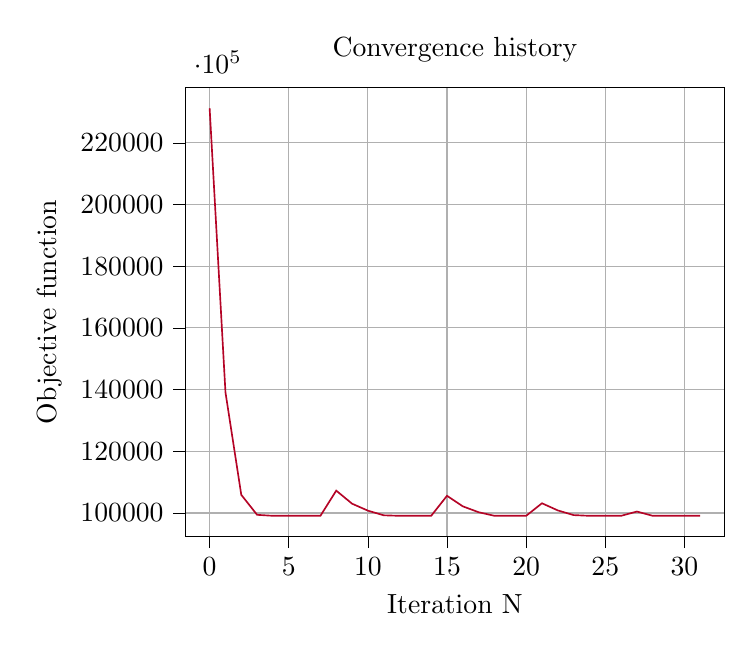
\begin{tikzpicture}

\definecolor{darkgray176}{RGB}{176,176,176}
\definecolor{firebrick180438}{RGB}{180,4,38}

\begin{axis}[
tick align=outside,
tick pos=left,
title={Convergence history},
x grid style={darkgray176},
xlabel={Iteration N},
xmajorgrids,
xmin=-1.55, xmax=32.55,
xtick style={color=black},
xtick={-5,0,5,10,15,20,25,30,35},
xticklabels={
  \(\displaystyle {\ensuremath{-}5}\),
  \(\displaystyle {0}\),
  \(\displaystyle {5}\),
  \(\displaystyle {10}\),
  \(\displaystyle {15}\),
  \(\displaystyle {20}\),
  \(\displaystyle {25}\),
  \(\displaystyle {30}\),
  \(\displaystyle {35}\)
},
y grid style={darkgray176},
ylabel={Objective function},
ymajorgrids,
ymin=92479.1843169952, ymax=237805.674226936,
ytick style={color=black},
ytick={80000,100000,120000,140000,160000,180000,200000,220000,240000},
yticklabels={
  \(\displaystyle {80000}\),
  \(\displaystyle {100000}\),
  \(\displaystyle {120000}\),
  \(\displaystyle {140000}\),
  \(\displaystyle {160000}\),
  \(\displaystyle {180000}\),
  \(\displaystyle {200000}\),
  \(\displaystyle {220000}\),
  \(\displaystyle {240000}\)
}
]
\addplot [semithick, firebrick180438]
table {%
0 231199.924685575
1 139115.71466262
2 105883.891802433
3 99406.9798995348
4 99085.9900030204
5 99084.934126946
6 99084.9341136118
7 99084.9341136118
8 107248.829074952
9 103020.371408933
10 100759.571286058
11 99250.5183147928
12 99084.9340849363
13 99084.9341136118
14 99084.9341136118
15 105581.687504654
16 102151.72910764
17 100245.402192191
18 99084.9338874528
19 99084.9341136118
20 99084.9341136118
21 103157.680865763
22 100837.744567021
23 99318.8277050646
24 99084.9340722716
25 99084.9341136118
26 99084.9341136118
27 100472.253237964
28 99084.9338583562
29 99084.9341136118
30 99084.9341136118
31 99084.9340098948
};
\end{axis}

\end{tikzpicture}
